\chapter{Uncertainty Quantification and Validation}
\label{ch:uq}

A quantitative estimate of the ion energy flux $\Gamma_{E}$ across a plasma sheath is only as useful as the confidence with which it is known. Every stage of the diagnostic-to-flux pipeline -- acquisition, calibration, inversion of a forward model to recover the ion velocity distribution function $f_{\mathrm{i}}(v)$, and moment integration to $\Gamma_{E}$ -- introduces its own uncertainty. A bare point estimate, without an error budget, is of limited value to an engineer sizing a plasma-facing component or a modeller reconciling simulation with experiment. This chapter treats uncertainty as a quantity to be propagated, tested, and validated with the same rigour as the flux estimate itself.

The chapter has four tasks: catalogue the sources of uncertainty in the measurement chain, each demanding different treatment; show how these propagate through the inverse problem mapping raw signals to $f_{\mathrm{i}}(v)$ and thence to $\Gamma_{E}$, via linearised and fully Bayesian formalisms, with correct interpretation of credible intervals; describe a validation methodology exercising the pipeline against synthetic signals from a known particle-in-cell (PIC) ground truth, isolating recovery error from the confounds of a real experiment; and address cross-diagnostic consistency, where independent diagnostics probing the same volume must agree within combined uncertainty. It closes with the benchmarking metrics and acceptance criteria used throughout the monograph to certify an inversion fit for quantitative use.

Notation follows earlier chapters: $T_{\mathrm{e}}$, $T_{\mathrm{i}}$ electron and ion temperatures; $n_{\mathrm{e}}$, $n_{\mathrm{i}}$ number densities; $\lambda_{\mathrm{D}}$ Debye length; $u_{\mathrm{B}}$ Bohm velocity; $f_{\mathrm{i}}(v)$ ion velocity distribution function; $\Gamma_{E}$ ion energy flux.

\section{Sources of Uncertainty}
\label{sec:uq-sources}

The total uncertainty on a reconstructed flux $\Gamma_{E}$ decomposes into three classes differing in statistical character and remedy: measurement noise, calibration uncertainty, and model error. These determine which uncertainties shrink with averaging, which need an independent reference standard, and which cannot be reduced without changing the physical model.

\subsection{Measurement Noise}
\label{subsec:meas-noise}

Measurement noise is the stochastic fluctuation in a recorded signal that persists even at fixed plasma state and calibration -- additive and uncorrelated between acquisitions to good approximation, so its effect shrinks with the number of samples averaged.

For a swept Langmuir probe, shot noise, amplifier Johnson noise, and RF/pulsed-power pickup contribute to trace variance, amplified substantially by the differentiation needed to extract an electron energy distribution. For LIF and RFEA measurements of $f_{\mathrm{i}}(v)$, photon-counting statistics and quantisation set an irreducible noise floor per channel. For incoherent Thomson scattering the fundamental source is Poisson statistics of scattered photons, compounded by stray light and dark counts; achievable accuracy on $T_{\mathrm{e}}$ and $n_{\mathrm{e}}$ is a long-studied problem \cite{ref0384,ref0355}. We model noise on channel $d_{k}$ as
\begin{equation}
d_{k} = M_{k}(\boldsymbol{\theta}) + \varepsilon_{k}, \qquad \varepsilon_{k} \sim \mathcal{N}\!\left(0, \sigma_{k}^{2}\right),
\label{eq:noise-model}
\end{equation}
where $M_{k}(\boldsymbol{\theta})$ is the noise-free forward-model prediction given plasma-state vector $\boldsymbol{\theta}$ (parametrising $f_{\mathrm{i}}(v)$ or its moments $n_{\mathrm{i}}$, $T_{\mathrm{i}}$, $T_{\mathrm{e}}$), and $\sigma_{k}^{2}$ is the channel noise variance. The Gaussian, zero-mean assumption is justified at high photon count, but can fail at low signal, where a Poisson likelihood is more appropriate (\cref{subsec:likelihood}).

Because measurement noise is uncorrelated across acquisitions, its contribution to a derived quantity scales as $1/\sqrt{N_{\text{shots}}}$, provided the plasma state is stationary over the averaging window -- unlike the other two classes, neither of which is reduced by repeated sampling under fixed calibration.

\subsection{Calibration Uncertainty}
\label{subsec:calib}

Calibration uncertainty arises from imperfect knowledge of the mapping between a raw reading and the physical quantity it represents -- the absolute sensitivity of a Thomson-scattering system, the transmission and linearity of an RFEA, the wavelength/intensity calibration of a spectrometer, or the collection solid angle and tip area of a Langmuir probe. Unlike measurement noise, it is systematic: it biases every measurement from a given instrument configuration in a correlated way that averaging cannot remove.

We represent it as a nuisance parameter (vector) $\boldsymbol{\kappa}$ entering the forward model alongside $\boldsymbol{\theta}$,
\begin{equation}
d_{k} = M_{k}(\boldsymbol{\theta}; \boldsymbol{\kappa}) + \varepsilon_{k},
\label{eq:calib-nuisance}
\end{equation}
with prior $p(\boldsymbol{\kappa})$ from an independent calibration campaign. Cross-calibration of one diagnostic against another -- e.g.\ anchoring a Thomson density scale against interferometry -- is central to the integrated data analysis philosophy of \cref{sec:cross-diagnostic} \cite{ref0707,ref0712}. Because $\boldsymbol{\kappa}$ is shared across a campaign rather than resampled shot to shot, its uncertainty enters as a correlated bias in every inferred flux, carried explicitly through the inversion (\cref{sec:propagation}) rather than estimated post hoc.

Table~\ref{tab:uncertainty-sources} summarises the three classes, their statistical behaviour, and their treatment in \cref{sec:propagation}, with magnitudes representative of typical practice rather than a specific experiment.

\begin{table}[htbp]
\centering
\caption{Illustrative taxonomy of uncertainty sources entering the ion-energy-flux inversion. Magnitudes are representative, not measured values from a specific experiment.}
\label{tab:uncertainty-sources}
\begin{tabular}{@{}p{2.6cm}p{4.6cm}p{2.4cm}p{3.6cm}@{}}
\toprule
Source & Physical origin & Typical relative magnitude & Propagation treatment \\
\midrule
Measurement noise & Photon shot noise, amplifier/Johnson noise, quantisation & \SI{2}{\percent}--\SI{15}{\percent} per shot & Likelihood covariance $\Sigma_{d}$; averages as $1/\sqrt{N_{\text{shots}}}$ \\
Calibration uncertainty & Absolute sensitivity, cross-section, geometric factors & \SI{5}{\percent}--\SI{20}{\percent} & Nuisance parameter $\boldsymbol{\kappa}$ with informative prior; marginalised \\
Model (structural) error & Truncated moment hierarchy, collisionality assumption, EEDF shape & problem-dependent, often \SI{10}{\percent}--\SI{30}{\percent} & Inflated likelihood variance, model-discrepancy term, or explicit alternative-model comparison \\
\bottomrule
\end{tabular}
\end{table}

\subsection{Model Error and Structural Uncertainty}
\label{subsec:model-error}

The third, most subtle class is model error -- the discrepancy between the forward model $M(\boldsymbol{\theta})$ and the true data-generating process, persisting even with noise-free, perfectly calibrated measurements. In the sheath/presheath context it stems from recurring simplifications: an assumed collisionless or weakly collisional presheath when collisionality is non-negligible; a Maxwellian or bi-Maxwellian EEDF when the true distribution is depleted at high energy; a planar, one-dimensional sheath model where geometry introduces multi-dimensional structure; and truncated moment hierarchies linking $f_{\mathrm{i}}(v)$ to the Bohm criterion and energy-flux integral. Kinetic-theoretic extensions of the Bohm criterion to collisional, magnetised, and non-Maxwellian plasmas show the idealised cold-fluid picture can shift the effective ion speed at the sheath edge, and hence the inferred flux.

Formally, the true data-generating process is
\begin{equation}
d_{k} = M_{k}(\boldsymbol{\theta}) + \delta_{k}(\boldsymbol{\theta}) + \varepsilon_{k},
\label{eq:model-discrepancy}
\end{equation}
where $\delta_{k}(\boldsymbol{\theta})$ is an unknown, deterministic model-discrepancy term -- if known exactly it would simply be absorbed into an improved forward model. Two strategies bound the resulting uncertainty: variance inflation, adding a term $\sigma_{\text{model},k}^{2}$ to the likelihood covariance calibrated from residual structure in synthetic closure tests (\cref{sec:synthetic-validation}); and multi-model comparison, repeating the inversion under distinct forward models and reporting the spread in $\Gamma_{E}$ as an added uncertainty band. Both are necessarily conservative rather than exact, since no data-driven procedure can fully characterise an unmodelled effect (\cref{sec:benchmarking}).

\subsection{Uncertainty Budget Synthesis}
\label{subsec:budget-synthesis}

The three contributions must be combined into a single budget on $\Gamma_{E}$. Because measurement noise and calibration uncertainty act through distinct mechanisms -- one shot-to-shot random, the other a shared systematic offset -- and model error is not random in the classical sense, a naive root-sum-square combination is exact only in the linear, Gaussian, independent-source limit. We propagate noise and calibration uncertainty jointly through the Bayesian inversion of \cref{sec:propagation}, encoded in the posterior covariance of $\Gamma_{E}$; model error is reported separately, as an explicitly flagged band, avoiding a deceptively tight error bar that reflects only instrument noise while ignoring the forward model's assumptions.

\section{Propagation of Uncertainty Through the Inversion}
\label{sec:propagation}

We now examine how these uncertainties propagate through the inverse problem mapping noisy, calibration-limited measurements $\mathbf{d} = (d_{1}, \dots, d_{K})$ to the plasma-state parameters $\boldsymbol{\theta}$ and, via the moment integral below, to $\Gamma_{E}$.

\subsection{Forward Model and Likelihood}
\label{subsec:likelihood}

This inversion is an instance of the ill-posed inverse problems pervading plasma diagnostics: a low-dimensional or continuous quantity ($f_{\mathrm{i}}(v)$ or a summary of it) must be recovered from finite, noisy indirect measurements through a frequently ill-conditioned forward operator -- the same tension between fidelity to noisy data and solution stability seen in tomographic and other regularised inverse problems.

Given the noise model of \cref{eq:noise-model} and noise covariance $\Sigma_{d} = \operatorname{diag}(\sigma_{1}^{2}, \dots, \sigma_{K}^{2})$, the likelihood of $\boldsymbol{\theta}$ given the data is
\begin{equation}
\mathcal{L}(\mathbf{d} \mid \boldsymbol{\theta}) = \frac{1}{(2\pi)^{K/2} |\Sigma_{d}|^{1/2}} \exp\!\left[-\tfrac{1}{2} \left(\mathbf{d} - M(\boldsymbol{\theta})\right)^{\mathsf{T}} \Sigma_{d}^{-1} \left(\mathbf{d} - M(\boldsymbol{\theta})\right)\right].
\label{eq:gaussian-likelihood}
\end{equation}
At low count rate, the likelihood is instead built from the Poisson probability mass function. In either case, the negative log-likelihood is a data-misfit functional minimised subject to regularisation stabilising the ill-posed problem -- a strategy long established in Tikhonov-regularised inversions \cite{ref0677,ref0692}.

\subsection{Bayesian Posterior and the Role of the Prior}
\label{subsec:bayesian-posterior}

Rather than a single regularised point estimate, we adopt a fully Bayesian strategy: $\boldsymbol{\theta}$ (and, where relevant, $\boldsymbol{\kappa}$) is a random variable whose posterior, conditioned on $\mathbf{d}$, is given by Bayes' theorem,
\begin{equation}
p(\boldsymbol{\theta} \mid \mathbf{d}) = \frac{\mathcal{L}(\mathbf{d} \mid \boldsymbol{\theta})\, p(\boldsymbol{\theta})}{\int \mathcal{L}(\mathbf{d} \mid \boldsymbol{\theta}')\, p(\boldsymbol{\theta}')\, \mathrm{d}\boldsymbol{\theta}'},
\label{eq:bayes-theorem}
\end{equation}
where $p(\boldsymbol{\theta})$ encodes physical constraints (positivity of $n_{\mathrm{i}}$, $T_{\mathrm{i}}$; monotonic decay of $f_{\mathrm{i}}(v)$ at large $|v|$) and prior information. This framing is well established across low-temperature and fusion diagnostics, from integrated data analysis \cite{ref0706,ref0707,ref0710,ref0713} and Bayesian inference from Thomson-scattering data \cite{ref0683} to Bayesian UQ of thruster and sheath models \cite{ref0719} and broader treatments \cite{ref0727,ref0711}.

The prior deserves particular care here, since inversion from a finite set of channels to a continuous $f_{\mathrm{i}}(v)$ is formally under-determined without regularisation, and the prior is the principled mechanism for introducing it. Where $f_{\mathrm{i}}(v)$ is non-parametric, a smoothness-penalising Tikhonov or total-variation prior is standard \cite{ref0692}; where parametric, the prior reduces to bounds and weak informative distributions on $n_{\mathrm{i}}$, $T_{\mathrm{i}}$, and drift velocity.

\subsection{Linearised Propagation: Jacobians and the Posterior Covariance}
\label{subsec:linearised}

Near the MAP estimate $\hat{\boldsymbol{\theta}}$, the posterior of \cref{eq:bayes-theorem} can be approximated as multivariate Gaussian via a local (Laplace) expansion of the log-posterior. Writing the Jacobian
\begin{equation}
J_{k j} = \left.\frac{\partial M_{k}(\boldsymbol{\theta})}{\partial \theta_{j}}\right|_{\boldsymbol{\theta} = \hat{\boldsymbol{\theta}}},
\label{ch21-eq:jacobian}
\end{equation}
the posterior covariance of $\boldsymbol{\theta}$ is
\begin{equation}
\Sigma_{\theta} \approx \left(J^{\mathsf{T}} \Sigma_{d}^{-1} J + \Sigma_{\text{prior}}^{-1}\right)^{-1},
\label{ch21-eq:posterior-cov}
\end{equation}
the Bayesian generalisation of the Cram\'er-Rao bound: for an uninformative prior ($\Sigma_{\text{prior}}^{-1} \to 0$) it reduces to the inverse Fisher information matrix $(J^{\mathsf{T}} \Sigma_{d}^{-1} J)^{-1}$. This propagation is inexpensive, needing only the Jacobian at a single point, and is the workhorse for routine, shot-by-shot error bars throughout this monograph.

To propagate $\Sigma_{\theta}$ onto $\Gamma_{E}$ we use the delta method: if $\Gamma_{E} = g(\boldsymbol{\theta})$ (the moment integral of \cref{eq:flux-moment} below), then, to leading order,
\begin{equation}
\sigma_{\Gamma_{E}}^{2} \approx \left(\nabla_{\boldsymbol{\theta}} g\right)^{\mathsf{T}} \Sigma_{\theta} \left(\nabla_{\boldsymbol{\theta}} g\right)\Big|_{\boldsymbol{\theta} = \hat{\boldsymbol{\theta}}}.
\label{eq:delta-method}
\end{equation}
The ion energy flux is defined as
\begin{equation}
\Gamma_{E} = \int_{0}^{\infty} \tfrac{1}{2} m_{\mathrm{i}} v^{2} \, v\, f_{\mathrm{i}}(v) \, \mathrm{d}v ,
\label{eq:flux-moment}
\end{equation}
so $g$ is a nonlinear functional of $f_{\mathrm{i}}(v)$, and $\nabla_{\boldsymbol{\theta}} g$ is evaluated with respect to whatever parametrisation enters $\boldsymbol{\theta}$. For a drifting Maxwellian at $T_{\mathrm{i}}$ with drift near the Bohm speed $u_{\mathrm{B}} = \sqrt{k_{\mathrm{B}} T_{\mathrm{e}} / m_{\mathrm{i}}}$, \cref{eq:flux-moment} reduces to $\Gamma_{E} \approx n_{\mathrm{i}} u_{\mathrm{B}} \left(\tfrac{1}{2} m_{\mathrm{i}} u_{\mathrm{B}}^{2} + \tfrac{5}{2} k_{\mathrm{B}} T_{\mathrm{i}}\right)$, a closed form whose uncertainty follows analytically via the delta method on $(n_{\mathrm{i}}, T_{\mathrm{e}}, T_{\mathrm{i}})$ -- a useful cross-check.

\subsection{Credible Intervals and Their Interpretation}
\label{subsec:credible}

A Bayesian $100(1-\alpha)\%$ credible interval for $\Gamma_{E}$, $\left[\Gamma_{E}^{\text{lo}}, \Gamma_{E}^{\text{hi}}\right]$, satisfies
\begin{equation}
\int_{\Gamma_{E}^{\text{lo}}}^{\Gamma_{E}^{\text{hi}}} p(\Gamma_{E} \mid \mathbf{d}) \, \mathrm{d}\Gamma_{E} = 1 - \alpha,
\label{eq:credible-interval}
\end{equation}
where $p(\Gamma_{E} \mid \mathbf{d})$ is the marginal posterior of the flux, from either the Gaussian approximation of \cref{eq:delta-method} or the sampling-based posterior of \cref{subsec:sampling}. A credible interval is not numerically identical to a frequentist confidence interval, though the two coincide asymptotically under a flat prior: the credible interval states the posterior probability that $\Gamma_{E}$ lies in the range \emph{given the data and assumed model}, whereas a confidence interval concerns long-run coverage frequency under repeated sampling. The distinction matters because validity depends on the correctness of the assumed likelihood and prior -- precisely what \cref{sec:synthetic-validation,sec:cross-diagnostic} probe. Where the equal-tailed interval is inconvenient for a strongly skewed posterior, we instead report the highest posterior density (HPD) interval, natural near the edge of the physically allowed space, where positivity constraints on $n_{\mathrm{i}}$ or $T_{\mathrm{i}}$ truncate it asymmetrically.

\subsection{Sampling-Based Propagation}
\label{subsec:sampling}

Linearised propagation is accurate only when the log-posterior is well approximated by a quadratic form near its maximum -- which can fail when $M(\boldsymbol{\theta})$ is strongly nonlinear, when the posterior is multimodal (e.g.\ a near-degeneracy between $T_{\mathrm{i}}$ and a drift velocity in a poorly resolved LIF line shape), or when physical bounds truncate it asymmetrically. We then characterise the full posterior by Markov-chain Monte Carlo (MCMC), drawing an ensemble $\{\boldsymbol{\theta}^{(1)}, \dots, \boldsymbol{\theta}^{(N)}\}$ from $p(\boldsymbol{\theta} \mid \mathbf{d})$ and propagating each through \cref{eq:flux-moment} to obtain $\{\Gamma_{E}^{(1)}, \dots, \Gamma_{E}^{(N)}\}$, from which the marginal posterior, credible intervals, and higher moments are estimated non-parametrically, standard practice in integrated data analysis \cite{ref0706}. Linearised propagation gives routine per-shot error bars; full sampling is reserved for validation studies, suspected multimodality, and the benchmarking exercises of \cref{sec:benchmarking}.

\begin{figure}[htbp]
\centering
\begin{tikzpicture}[
 node distance=0.9cm and 1.6cm,
 box/.style={draw, thick, align=center, minimum width=2.6cm, minimum height=1.0cm, font=\small},
 arr/.style={-{Stealth[length=2.2mm]}, thick}
]
\node[box] (diag) {Diagnostic\\signals $\mathbf{d}$};
\node[box, right=of diag] (fwd) {Forward model\\$M(\boldsymbol{\theta};\boldsymbol{\kappa})$\\+ noise/calib.\\uncertainty};
\node[box, right=of fwd] (post) {Bayesian\\posterior\\$p(\boldsymbol{\theta}\mid\mathbf{d})$};
\node[box, right=of post] (flux) {Moment\\integral\\$\Gamma_{E}=g(\boldsymbol{\theta})$};
\node[box, below=of post] (val) {Synthetic (PIC)\\validation \&\\cross-diagnostic\\residuals};
\draw[arr] (diag) -- (fwd);
\draw[arr] (fwd) -- (post);
\draw[arr] (post) -- (flux);
\draw[arr] (val) -- (post) node[midway, right, align=left, font=\scriptsize] {calibrates\\model \& prior};
\draw[arr] (flux.south) .. controls +(0,-0.9) and +(1.3,-0.9) .. (val.east);
\end{tikzpicture}
\caption{Schematic (illustrative, not derived from a specific dataset) of the pipeline: diagnostic channels enter a forward model carrying explicit noise and calibration uncertainty; Bayesian inversion yields a posterior over the plasma state, from which $\Gamma_{E}$ follows by moment integration; synthetic PIC validation and cross-diagnostic residuals feed back to calibrate the model and prior.}
\label{fig:uq-pipeline}
\end{figure}

\section{Synthetic Validation Against PIC Ground Truth}
\label{sec:synthetic-validation}

\subsection{Rationale for Synthetic Closure Tests}
\label{subsec:synthetic-rationale}

The credible intervals of \cref{sec:propagation} are trustworthy only insofar as the assumed likelihood, prior, and forward model reflect the true measurement process. Because the ground-truth flux is never known exactly in a real experiment, inversion fidelity cannot be assessed from experimental data alone: any discrepancy between reconstructed $\Gamma_{E}$ and an independent reference is degenerate between inversion error, forward-model error, and reference measurement error. PIC simulation breaks this degeneracy -- a PIC run of the sheath and presheath provides a self-consistent, fully specified $f_{\mathrm{i}}^{\text{PIC}}(v)$ at every location and time, from which $\Gamma_{E}^{\text{PIC}}$ follows directly from \cref{eq:flux-moment} with no measurement error. Forward-modelling what a probe, RFEA, or Thomson system would record from this known $f_{\mathrm{i}}^{\text{PIC}}(v)$, and adding synthetic noise and calibration error consistent with \cref{sec:uq-sources}, yields a closure test against a known answer, mirroring the practice in fusion integrated data analysis of validating Bayesian frameworks against synthetic data before real discharges \cite{ref0706,ref0712}. Continuum and PIC kinetic simulations resolve full ion and electron kinetics without the fluid closures being tested.

\subsection{Construction of Synthetic Diagnostic Data}
\label{subsec:synthetic-construction}

A synthetic study proceeds in four steps: run a PIC simulation to a stationary state and extract $f_{\mathrm{i}}^{\text{PIC}}(v)$ at the diagnostic location(s), with corresponding $n_{\mathrm{e}}$, $n_{\mathrm{i}}$, $T_{\mathrm{e}}$, $\lambda_{\mathrm{D}}$; compute the true flux $\Gamma_{E}^{\text{PIC}}$ by direct integration of \cref{eq:flux-moment}; apply each diagnostic's forward model to $f_{\mathrm{i}}^{\text{PIC}}(v)$ to generate the noise-free signal $M_{k}(\boldsymbol{\theta}^{\text{PIC}})$, then add synthetic noise $\varepsilon_{k}$ and, where applicable, a calibration offset from $p(\boldsymbol{\kappa})$, reproducing \cref{eq:noise-model}--\cref{eq:calib-nuisance} with a known ground truth; and pass $\mathbf{d}^{\text{synth}}$ through the full, unmodified inversion pipeline to obtain $p(\boldsymbol{\theta} \mid \mathbf{d}^{\text{synth}})$ and a reconstructed flux $\hat{\Gamma}_{E}$ with its credible interval.

This is repeated over independent noise realisations at fixed $\boldsymbol{\theta}^{\text{PIC}}$, and separately over distinct plasma conditions spanning the parameter space ($T_{\mathrm{e}}/T_{\mathrm{i}}$, neutral pressure, magnetisation), probing both statistical calibration and robustness across the diagnostic suite's operating envelope.

\subsection{Recovery of the Known Flux}
\label{subsec:recovery}

For each realisation $r = 1, \dots, R$, the reconstruction error is
\begin{equation}
e_{r} = \hat{\Gamma}_{E}^{(r)} - \Gamma_{E}^{\text{PIC}},
\label{eq:recon-error}
\end{equation}
characterised by its mean (bias) and standard deviation,
\begin{equation}
\overline{e} = \frac{1}{R} \sum_{r=1}^{R} e_{r}, \qquad
s_{e}^{2} = \frac{1}{R-1} \sum_{r=1}^{R} \left(e_{r} - \overline{e}\right)^{2}.
\label{eq:bias-scatter}
\end{equation}
A well-behaved inversion exhibits $\overline{e}$ consistent with zero, $|\overline{e}| \lesssim s_{e} / \sqrt{R}$; a significant nonzero $\overline{e}$ indicates systematic bias requiring diagnosis before deployment. The scatter $s_{e}$ gives an independent check on credible-interval width, formalised as a coverage test in \cref{subsec:coverage}, mirroring UQ studies of thruster and sheath models against synthetic ground truth \cite{ref0719,ref0712}.

\subsection{Coverage and Calibration of the Posterior}
\label{subsec:coverage}

The single most informative diagnostic is coverage probability: for a nominal $100(1-\alpha)\%$ credible interval, the fraction of realisations where $\Gamma_{E}^{\text{PIC}}$ falls inside $\left[\Gamma_{E}^{\text{lo},(r)}, \Gamma_{E}^{\text{hi},(r)}\right]$ should, over a large ensemble, converge to $1-\alpha$:
\begin{equation}
\widehat{C}(1-\alpha) = \frac{1}{R} \sum_{r=1}^{R} \mathbb{1}\!\left[\Gamma_{E}^{\text{lo},(r)} \le \Gamma_{E}^{\text{PIC}} \le \Gamma_{E}^{\text{hi},(r)}\right],
\label{eq:coverage}
\end{equation}
with $\mathbb{1}[\cdot]$ the indicator function. Coverage below nominal ($\widehat{C} < 1-\alpha$) indicates overconfident, too-narrow intervals, typically from unmodelled model error (\cref{subsec:model-error}) not folded into the likelihood variance; $\widehat{C} > 1-\alpha$ indicates conservative, overly broad intervals. Plotting $\widehat{C}(1-\alpha)$ against $1-\alpha$ produces a calibration curve; a perfectly calibrated inversion traces the diagonal. Systematic departures trigger a revisit of \cref{subsec:model-error}, pinpointing where the uncertainty budget fails to capture the true error.

\section{Cross-Diagnostic Consistency and Residual Analysis}
\label{sec:cross-diagnostic}

\subsection{Independent Diagnostic Channels}
\label{subsec:independent-channels}

Synthetic validation establishes internal consistency of a single diagnostic's pipeline, but cannot detect a model error common to both the PIC forward model and the inversion's forward model -- e.g.\ an incorrect ion-neutral collision cross-section used in both. A complementary check is available whenever two or more independent diagnostics probe the same volume: a Langmuir probe and Thomson system measuring $T_{\mathrm{e}}$, $n_{\mathrm{e}}$ in the same discharge, or an RFEA and LIF system both probing $f_{\mathrm{i}}(v)$ near the sheath edge. Because these rely on distinct physical mechanisms, they are subject to largely uncorrelated systematic errors, so their mutual agreement, or disagreement, is strong and independent evidence about the underlying model -- a role long served by direct comparisons of Langmuir-probe and Thomson-scattering $T_{\mathrm{e}}$, $n_{\mathrm{e}}$, and one that extends naturally to the ion energy flux itself.

\subsection{Residual Definition and Whitening}
\label{subsec:residual-def}

For diagnostics $A$ and $B$ independently estimating the same $\Gamma_{E}$ (or a shared plasma-state parameter feeding into it), the cross-diagnostic residual is
\begin{equation}
r_{AB} = \frac{\hat{\Gamma}_{E}^{A} - \hat{\Gamma}_{E}^{B}}{\sqrt{\sigma_{A}^{2} + \sigma_{B}^{2} - 2\,\operatorname{cov}(A,B)}},
\label{eq:cross-residual}
\end{equation}
where $\sigma_{A}$, $\sigma_{B}$ are the marginal posterior standard deviations, and $\operatorname{cov}(A,B)$ any covariance from a shared calibration parameter or plasma-state estimate. This whitening converts the residual into a quantity that should be distributed $r_{AB} \sim \mathcal{N}(0,1)$ if both diagnostics' forward models and uncertainty budgets are correct, following standard integrated data analysis practice of jointly modelling multiple channels within a single Bayesian graph \cite{ref0713,ref0683}.

It is often more informative to examine the full residual vector across every channel -- the whitened data misfit $\Sigma_{d}^{-1/2}\left(\mathbf{d} - M(\hat{\boldsymbol{\theta}})\right)$ at the posterior mode -- which under a correctly specified model should have zero mean, unit variance per component, and no structure correlated with a control variable such as probe position, discharge time, or wavelength; a normality test or quantile-quantile plot gives a compact summary.

\subsection{Detecting Model Misspecification}
\label{subsec:misspecification}

Residual analysis is valuable less for confirming a model correct -- no finite test can fully establish that -- than for revealing how it is wrong. A residual pattern correlated with a physical control variable is informative: a trend in $r_{AB}$ with neutral gas pressure suggests an unmodelled collisional term in the presheath model; a trend with probe bias voltage in a Langmuir-derived $T_{\mathrm{e}}$ suggests sheath expansion or secondary-electron-emission effects; a trend with scattering angle in a Thomson-derived $T_{\mathrm{e}}$ can reveal an uncorrected instrument-function artefact \cite{ref0360}. Such analysis is diagnostic of the functional form of the missing physics, not merely its magnitude: inflation absorbs an effect's size into a wider interval, but only structured residual analysis points toward the correction that removes the discrepancy at its source. Any significant residual trend therefore mandates model revision -- returning to \cref{subsec:model-error} and, where necessary, a revised PIC-based validation campaign -- rather than being absorbed silently into a larger reported uncertainty.

\section{Benchmarking Metrics and Acceptance Criteria}
\label{sec:benchmarking}

Building on the propagation methodology and the two validation strategies above -- synthetic closure against PIC ground truth, and empirical cross-diagnostic consistency -- we define a compact set of metrics against which any inversion pipeline is benchmarked before acceptance for quantitative use.

\subsection{Point-Estimate Accuracy Metrics}
\label{subsec:point-metrics}

Three point-estimate metrics, from the synthetic-validation ensemble of \cref{sec:synthetic-validation}, quantify accuracy independent of reported uncertainty. Normalised bias,
\begin{equation}
B_{\Gamma} = \frac{\overline{e}}{\Gamma_{E}^{\text{PIC}}},
\label{eq:norm-bias}
\end{equation}
quantifies systematic offset relative to true flux magnitude; normalised RMSE,
\begin{equation}
\text{RMSE}_{\Gamma} = \frac{1}{\Gamma_{E}^{\text{PIC}}}\sqrt{\frac{1}{R}\sum_{r=1}^{R} e_{r}^{2}},
\label{eq:rmse}
\end{equation}
combines bias and scatter into a single figure of merit; and reduced chi-squared at the posterior mode,
\begin{equation}
\chi_{\nu}^{2} = \frac{1}{\nu} \left(\mathbf{d} - M(\hat{\boldsymbol{\theta}})\right)^{\mathsf{T}} \Sigma_{d}^{-1} \left(\mathbf{d} - M(\hat{\boldsymbol{\theta}})\right),
\label{eq:chi2}
\end{equation}
with $\nu = K - \dim(\boldsymbol{\theta})$, gives a per-shot goodness-of-fit near unity for a well-specified model; values persistently above unity indicate underestimated noise or unmodelled structure, values below unity an over-flexible model fitting noise.

\subsection{Distributional and Coverage Metrics}
\label{subsec:distributional-metrics}

Point-estimate metrics alone cannot certify an uncertainty-aware diagnostic, since a pipeline can achieve excellent RMSE while misreporting its uncertainty. We therefore also report the coverage calibration curve and its scalar summary,
\begin{equation}
\text{CCE} = \int_{0}^{1} \left|\widehat{C}(1-\alpha) - (1-\alpha)\right| \, \mathrm{d}\alpha,
\label{eq:cce}
\end{equation}
the mean absolute deviation of the empirical coverage curve from the ideal diagonal. We also report cross-diagnostic residual statistics (\cref{subsec:residual-def}): mean and standard deviation of $r_{AB}$ across available pairs, and the outlier fraction $|r_{AB}| > 2$, which under the standard-normal null should not exceed about \SI{5}{\percent}.

\begin{table}[htbp]
\centering
\caption{Benchmarking metrics used to certify the ion-energy-flux inversion pipeline, with acceptance criteria applied throughout this monograph. Thresholds are working criteria for this project, not values from a prior publication.}
\label{tab:acceptance-criteria}
\begin{tabular}{@{}p{2.8cm}p{5.4cm}p{4.4cm}@{}}
\toprule
Metric & Definition & Acceptance criterion \\
\midrule
Normalised bias $B_{\Gamma}$ & Mean synthetic reconstruction error, \cref{eq:norm-bias} & $|B_{\Gamma}| < \num{0.05}$ \\
Normalised RMSE & Root-mean-square synthetic error, \cref{eq:rmse} & $\text{RMSE}_{\Gamma} < \num{0.15}$ \\
Reduced $\chi^{2}_{\nu}$ & Data misfit at posterior mode, \cref{eq:chi2} & $\num{0.7} < \chi_{\nu}^{2} < \num{1.5}$ \\
Coverage calibration error & Deviation of coverage curve from ideal, \cref{eq:cce} & $\text{CCE} < \num{0.05}$ \\
Cross-diagnostic residual & Whitened discrepancy between independent diagnostics, \cref{eq:cross-residual} & $|\overline{r_{AB}}| < \num{1}$; outlier fraction $< \SI{5}{\percent}$ \\
\bottomrule
\end{tabular}
\end{table}

\subsection{Acceptance Criteria for Deployment}
\label{subsec:acceptance}

Table~\ref{tab:acceptance-criteria} collects the five metrics with the numerical thresholds adopted throughout the monograph. These are working engineering criteria calibrated to the accuracy needed for the intended application (comparative assessment of plasma-facing-component erosion and heat loading), not universal statistical constants; a stricter or looser set may suit a different application. An inversion configuration -- forward model, prior, and diagnostic hardware together -- is accepted for quantitative reporting only when it satisfies all five criteria across the synthetic-validation ensemble and, where available, the cross-diagnostic data set. On failure, the prescribed sequence is: verify $\Sigma_{d}$ is correctly estimated (a common cause of $\chi_{\nu}^{2}$ far from unity); examine the coverage curve and residual structure (\cref{subsec:coverage,subsec:misspecification}) for a specific missing effect; revisit the model-discrepancy treatment of \cref{subsec:model-error}; and, failing that, treat the configuration as unsuitable until the deficiency is resolved. This staged protocol lets flux estimates elsewhere in the monograph carry a defensible, independently tested claim to quantitative accuracy.

\begin{figure}[htbp]
\centering
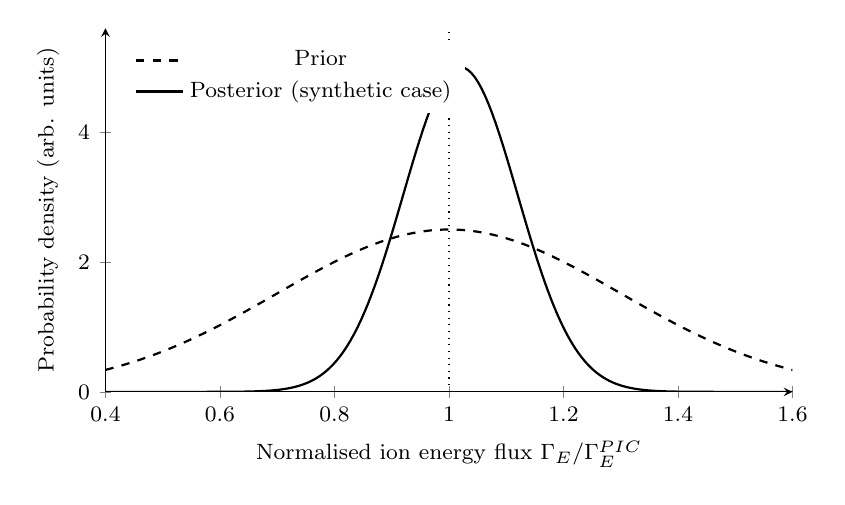
\begin{tikzpicture}
\begin{axis}[
 width=0.85\textwidth, height=6.2cm,
 xlabel={Normalised ion energy flux $\Gamma_{E}/\Gamma_{E}^{\text{PIC}}$},
 ylabel={Probability density (arb. units)},
 xmin=0.4, xmax=1.6, ymin=0, ymax=5.6,
 domain=0.4:1.6, samples=200,
 axis lines=left,
 legend pos=north west,
 legend style={font=\footnotesize, draw=none},
 tick label style={font=\footnotesize},
 label style={font=\footnotesize}
]
\addplot[thick, dashed, black] {2.5*exp(-0.5*((x-1.0)/0.30)^2)};
\addlegendentry{Prior}
\addplot[thick, black] {5.0*exp(-0.5*((x-1.02)/0.10)^2)};
\addlegendentry{Posterior (synthetic case)}
\draw[thin, dotted] (axis cs:1,0) -- (axis cs:1,5.6);
\end{axis}
\end{tikzpicture}
\caption{Schematic illustration (analytic Gaussian curves, not fitted to data) of the narrowing of the credible interval on $\Gamma_{E}$ upon Bayesian conditioning, for a representative synthetic case with true flux at normalised value $1$: a broad prior (dashed) updates into a substantially narrower posterior (solid), whose mode lies close to the known ground truth.}
\label{fig:posterior-narrowing}
\end{figure}

\section{Summary}
\label{sec:uq-summary}

This chapter developed the uncertainty-quantification and validation framework underlying every quantitative flux estimate in this monograph. We decomposed the uncertainty budget into measurement noise, calibration uncertainty, and model error, each requiring distinct treatment: additive noise covariance in the likelihood, informative priors on shared nuisance parameters, and either variance inflation or multi-model comparison for effects the forward model does not capture. We derived propagation through the Bayesian inversion -- from the likelihood through the posterior of \cref{eq:bayes-theorem}, its linearised Laplace/delta-method propagation onto $\Gamma_{E}$, to full sampling-based characterisation when linearity cannot be assumed -- and clarified the interpretation of credible intervals. We described a synthetic closure-test methodology exercising the complete pipeline against signals from a known PIC ground truth, quantifying reconstruction bias and scatter and, critically, calibrating credible intervals via empirical coverage probability. We complemented this with cross-diagnostic consistency analysis, in which whitened residuals between independent diagnostics expose misspecification a single-diagnostic test cannot detect. Finally, we consolidated these strands into five benchmarking metrics -- normalised bias, normalised RMSE, reduced chi-squared, coverage calibration error, and cross-diagnostic residual consistency -- with explicit acceptance criteria: the gate every inversion configuration must pass before its flux estimates are reported as quantitatively reliable, error bars that are not merely computed, but tested.
